\documentclass[twocolumn, 10pt]{article}
\usepackage{fullpage}
\usepackage[top=2cm, bottom=4cm, left=2cm, right=2cm]{geometry}
\usepackage{amsmath,amsthm,amsfonts,amssymb,amscd}
\usepackage{lastpage}
\usepackage{enumerate}
\usepackage{enumitem}
\usepackage{fancyhdr}
\usepackage{mathrsfs}
\usepackage{xcolor}
\usepackage{graphicx}
\usepackage{csvsimple}
\usepackage{booktabs}
\usepackage{tabularx}
\usepackage{listings}
\usepackage{hyperref}
\usepackage{mathtools}
\usepackage{tikz} % for graphics
\usepackage{yquant} % works with tikz; for quantum circuits
\usepackage{textcomp}
\usepackage{circuitikz} % for classical circuits
\usepackage{quantikz}
\usetikzlibrary{positioning,arrows.meta,shapes.geometric,decorations.pathmorphing,calc}
\usepackage[normalem]{ulem}
\usepackage{upgreek}
\usepackage{contour}
\usepackage{comment}
\usepackage{ragged2e}
\usepackage{qtree}
\usepackage{float}
\usepackage{subcaption}
\newfloat{Code}{htbp}{loc}
\newcommand{\Codeautorefname}{Code}
\usepackage[
    backend=biber,
    style=numeric,
]{biblatex}
\addbibresource{refs.bib}
\usepackage[executable=venv/bin/python3]{pyluatex}

% ---- Include Custom Photonics TikZ Library ----
% tikz_photonics.tex
% A custom TikZ library for standard photonics components.
% Usage: \pic at (x,y) {photonics_laser={Label}};
%        \pic at (x,y) {photonics_polarizer={Label}};   (angle in optional key)
%        \pic at (x,y) {photonics_bs={Label}};
%        \pic at (x,y) {photonics_fiber_bs={Label}};
%        \pic at (x,y) {photonics_apd={Label}};
\tikzset{
    photonics_laser/.pic={
        \draw[thin, fill=red!15] (-0.6,-0.1) rectangle (0.6,0.1);
        \node[above, font=\tiny\bfseries] at (0,0.1) {#1};
    },
    photonics_bs/.pic={
        \draw (-0.3,-0.3) rectangle (0.3,0.3);
        \draw (-0.3,-0.3) -- (0.3,0.3);
        \node[above left, font=\tiny] at (-0.3, 0.3) {#1};
    },
    photonics_mirror_bsp_right/.pic={
        \draw[thick, fill=gray!20] (-0.4, -0.05) rectangle (0.4, 0.05);
        \foreach \x in {-0.3,-0.1,0.1,0.3} \draw[thin, gray] (\x, -0.05) -- (\x+0.1, -0.2);
        \node[anchor=north west, font=\tiny, xshift=5pt, yshift=-5pt] {#1};
    },
    photonics_mirror_bsp_left/.pic={
        \draw[thick, fill=gray!20] (-0.4, -0.05) rectangle (0.4, 0.05);
        \foreach \x in {-0.3,-0.1,0.1,0.3} \draw[thin, gray] (\x, -0.05) -- (\x-0.1, -0.2);
        \node[anchor=north east, font=\tiny, xshift=-5pt, yshift=-5pt] {#1};
    },
    photonics_mirror_planar/.pic={
        \draw[line width=3pt,gray!40] (-0.35,0) -- (0.35,0);
        \draw[line width=1pt,gray] (-0.35,0) -- (0.35,0);
        \foreach \x in {-0.3,-0.15,0,0.15,0.3} \draw[line width=0.5pt,gray!60] (\x,0) -- (\x-0.08,-0.08);
        \node[anchor=south west, font=\tiny, xshift=2pt, yshift=2pt] {#1};
    },
    photonics_mirror_concave/.pic={
        \draw[thick, fill=gray!20] (-0.4,0) arc[start angle=150, end angle=30, radius=0.46] -- (0.4,0.05) -- (-0.4,0.05) -- cycle;
        \foreach \x in {-0.3,-0.1,0.1,0.3} \draw[thin, gray] (\x, 0.05) -- (\x-0.1, 0.2);
        \node[anchor=south east, font=\tiny, xshift=-5pt, yshift=5pt] {#1}; % M4 (Concave...)
    },
    photonics_photodiode/.pic={
        \draw[thick, fill=green!60!black] (0,0) circle (3pt);
        \node[right, font=\tiny, text=black, xshift=3pt] {#1};
    },
    % Standard APD label alias
    photonics_apd/.pic={
        \draw[thick, fill=green!60!black] (0,0) circle (3pt);
        \node[right, font=\tiny, text=black, xshift=3pt] {#1};
    },
    % Polarizer: circle with a diameter line indicating the transmission axis.
    % Convention follows Hecht "Optics" and Saleh & Teich "Fundamentals of Photonics".
    % Optional argument rotates the transmission-axis line (default = 0 deg = horizontal).
    photonics_polarizer/.pic={
        \draw[thick] (0,0) circle (0.28);
        % Draw transmission axis as a diameter; 45deg is the classic "diagonal polarizer" icon
        \draw[thick] ({-0.28*cos(45)},{-0.28*sin(45)}) -- ({0.28*cos(45)},{0.28*sin(45)});
        \node[above, font=\tiny, yshift=2pt] at (0,0.28) {#1};
    },
    % Fiber beam splitter: a rounded rectangle with "50/50" label
    photonics_fiber_bs/.pic={
        \draw[thick, rounded corners=3pt, fill=gray!20] (-0.4,-0.2) rectangle (0.4,0.2);
        \node[font=\tiny\bfseries] at (0,0) {50/50};
        \node[above, font=\tiny, yshift=1pt] at (0,0.2) {#1};
    },
}


% ---- Python code listing style ----
\lstset{
  language=Python,
  basicstyle=\ttfamily\scriptsize,
  keywordstyle=\color{blue!70!black}\bfseries,
  commentstyle=\color{gray}\itshape,
  stringstyle=\color{orange!80!black},
  showstringspaces=false,
  breaklines=true,
  breakatwhitespace=true,
  frame=single,
  framesep=3pt,
  rulecolor=\color{black!20},
  backgroundcolor=\color{black!3},
  numbers=left,
  numberstyle=\tiny\color{gray},
  numbersep=5pt,
  xleftmargin=12pt,
  captionpos=b,
}
\usepackage{fancyvrb}
\usepackage{etoolbox}
\usepackage{luacode}  % provides \begin{luacode}...\end{luacode} for safe Lua in preamble
\usepackage[disable]{todonotes}

% ── Guidance-comment toggle ──────────────────────────────────────────────────
% Set \showguidancetrue  to show the inline how-to comments in each section.
% Set \showguidancefalse to suppress them entirely (for the final submission).
% The `comment` package (loaded above) provides includecomment/excludecomment.
\newif\ifshowguidance
\showguidancetrue          % <─── flip to \showguidancefalse before submitting
\ifshowguidance
  \includecomment{guidance}
\else
  \excludecomment{guidance}
\fi

% \pythoncode[caption]{file}{label} — wraps in a Code float
\newcommand{\pythoncode}[3][]{%
  \begin{Code}[h]
    \vspace{2pt}%
    \lstinputlisting[language=Python]{#2}%
    \pyfileq{#2}%
    \vspace{2pt}%
    \ifx\relax#1\relax\else\caption{#1}\fi
    \ifx\relax#3\relax\else\label{#3}\fi
  \end{Code}%
}

\newcommand{\pythonsnippet}[3][]{%
  \begin{Code}[h]
    \vspace{2pt}%
    \lstinputlisting[language=Python]{#2}%
    \vspace{2pt}%
    \ifx\relax#1\relax\else\caption{#1}\fi
    \ifx\relax#3\relax\else\label{#3}\fi
  \end{Code}%
}

\newcommand{\pysnippetmethod}[4][]{%
  \pyc{import sys; sys.path.append('pycode') if 'pycode' not in sys.path else None; import extract; extract.extract_method('#2', '#3', 'pycode/tmp_snippet.py')}
  \begin{Code}[H]
    \vspace{2pt}%
    \lstinputlisting[language=Python]{pycode/tmp_snippet.py}%
    \vspace{2pt}%
    \ifx\relax#1\relax\else\caption{#1}\fi
    \ifx\relax#4\relax\else\label{#4}\fi
  \end{Code}%
}

% ─── Math helpers ──────────────────────────────────────────────────────────
\newcommand{\Arg}{\textrm{Arg}}
\def\res{\mathop{\textrm{Res}}\limits}
\newcommand{\Mod}[1]{\ (\mathrm{mod}\ #1)}
\DeclareMathOperator{\lcm}{lcm}
\providecommand{\bra}[1]{\langle #1|}
\providecommand{\ket}[1]{|#1\rangle}
\providecommand{\braket}[2]{\langle #1|#2\rangle}
\DeclareMathOperator{\Span}{Span}
\DeclareMathOperator{\trace}{tr}
\DeclareMathOperator{\rank}{rank}
\DeclareMathOperator{\nl}{null}
\DeclarePairedDelimiterX{\inpr}[2]{\langle}{\rangle}{#1\,,\,\mathopen{}#2}
\DeclareMathOperator{\img}{Im}
\newcommand{\fqed}{\relax\ifmmode\tag*{$\blacksquare$}\else\hfill$\blacksquare$\fi}
\newcommand{\iqed}{\relax\ifmmode\tag*{$\square$}\else\hfill$\square$\fi}
\newcommand*\makeAlph[1]{\symbol{\numexpr97+#1}}
\renewcommand{\thesection}{\Roman{section}}

% ─── CSV data table ─────────────────────────────────────────────────────────
% \csvdatatable{file}{caption}{label}{col-spec}{header-row}{data-row}
\newcommand{\csvdatatable}[6]{%
  \begin{table}[H]
    \centering\footnotesize
    \renewcommand{\arraystretch}{1.1}
    \csvreader[
      tabular={#4},
      head to column names,
      table head={\toprule #5},
      table foot=\bottomrule,
      late after line=\\,
    ]{#1}{}{#6}
    \caption{#2}
    \label{#3}
  \end{table}
}

% ─── BOM table (full, spans both columns) ──────────────────────────────────
% \bomtable{csv-file}{caption}{label}
% CSV must have columns: Category, Component, Part Number, Notes, Lab
% The Notes column uses tabularx X type for text wrapping.
\newcommand{\bomtable}[3]{%
  \begin{table*}[t]
    \centering\footnotesize
    \caption{#2}\label{#3}
    \renewcommand{\arraystretch}{1.15}
    \begin{tabularx}{\linewidth}{llp{1.6cm}X}\toprule
      Category & Component & Model & Specifications \\\midrule
      \csvreader[late after line=\\]{#1}%
        {Category=\Cat,Component=\Comp,Model=\Model,Specs=\Specs}%
        {\Cat & \Comp & \Model & \Specs}%
      \\\bottomrule
    \end{tabularx}
  \end{table*}
}

% ─── Component list (filtered by Lab column) ───────────────────────────────
% \componentlist{lab-tag}{csv-file}
%   lab-tag: value in the 5th CSV column, or "all" to include everywhere.
%   Renders as an itemize list: Component — Part# (first note clause)
%
% Uses \begin{luacode}...\end{luacode} (from the luacode package) so that
% LaTeX does NOT scan the Lua body for active characters (', ", etc.).
\begin{luacode}
function tex_componentlist(labparam, csvpath)
  local f = io.open(csvpath, "r")
  if not f then
    tex.sprint("\\emph{(BOM file not found: " .. csvpath .. ")}")
    return
  end
  local _header = f:read("*l")
  local out = {}
  for line in f:lines() do
    local raw = {}
    local inside = false
    local cur = ""
    for ch in (line .. ","):gmatch(".") do
      if ch == '"' then
        inside = not inside
      elseif ch == "," and not inside then
        raw[#raw + 1] = cur:match("^%s*(.-)%s*$")
        cur = ""
      else
        cur = cur .. ch
      end
    end
    local lab  = raw[5] or ""
    -- If lab column is empty or "all", it matches anything requested as "all"
    if lab == labparam or lab == "all" or (lab == "" and labparam == "all") then
      local comp  = raw[2] or ""
      local model = raw[3] or ""
      local specs = raw[4] or ""
      local entry = "\\textbf{" .. comp .. "}"
      local detail = ""
      if specs ~= "" then detail = specs end
      if model ~= "" then
        if detail ~= "" then detail = detail .. ", " .. model
        else detail = model end
      end
      if detail ~= "" then
        entry = entry .. " \\textit{(" .. detail .. ")}"
      end
      out[#out + 1] = "\\item " .. entry
    end
  end
  f:close()
  if #out > 0 then
    tex.sprint("\\begin{itemize}[noitemsep,topsep=2pt,leftmargin=1.6em]")
    for _, s in ipairs(out) do tex.sprint(s) end
    tex.sprint("\\end{itemize}")
  end
end
\end{luacode}
% ─── Lab tag macros ──────────────────────────────────────────────────────────
% Define sub-experiment tags here; use them in \componentlist{\laball}{...}
% All rows with tag "all" always appear regardless of which \labtagX is requested.
%
\newcommand{\laball}{all}         % included in every sub-experiment
% \newcommand{\labtagA}{part-a}   % uncomment and rename for each sub-experiment
% \newcommand{\labtagB}{part-b}
%
\newcommand{\componentlist}[2]{%
  \directlua{tex_componentlist(\luastring{#1}, \luastring{#2})}%
}

% ───────────────────────────────────────────────────────────────────────────
\title{Course CODE — [Lab Title]}
\author{[Author Names]}
\date{\today}

\begin{document}
\maketitle

\begin{abstract}
[Insert Abstract Here]
\end{abstract}

\begin{guidance}
\textit{\color{gray!60!black}\small\textbf{Abstract guidance:}
  State what was done, the key methods, and your main quantitative result(s).
  Avoid jargon; assume a reader who knows undergraduate physics.
  Do not start with ``In this paper\ldots''.}
\end{guidance}

% ===========================================================================
\section{Introduction}
% ===========================================================================
\begin{guidance}
\textit{\color{gray!60!black}\small\textbf{Introduction guidance:}
  Explain why this experiment is relevant.
  Give a one-sentence outline of each section; state your key result up front
  (PRL style: state the main result in the first paragraph, not as a surprise at the end).
  Cite the theoretical framework and any prior experimental results.}
\end{guidance}
[Insert Introduction Here]

% ===========================================================================
\section{Theory}
\label{sec:theory}
% ===========================================================================
\begin{guidance}
\textit{\color{gray!60!black}\small\textbf{Theory guidance:}
  Explain what you are testing theoretically.
  Derive or state the model(s) used to analyze your data.
  For each fitting function, give its equation and explain every parameter.
  Include theoretical predictions your results can be compared against.
  Discuss limiting cases (ideal vs.\ mixed state, classical vs.\ QM) where relevant.}
\end{guidance}
[Insert Theory Here]

% ===========================================================================
\section{Experimental Procedure}
% ===========================================================================
\begin{guidance}
\textit{\color{gray!60!black}\small\textbf{Procedure guidance:}
  Describe the apparatus clearly enough that a competent physicist could
  reproduce your results. Include:
  \begin{itemize}[noitemsep,topsep=2pt]
    \item A TikZ/figure diagram of the optical/electronic setup.
    \item The equipment list (use \texttt{\textbackslash componentlist}).
    \item Step-by-step alignment and acquisition protocol.
    \item Any deviations from the stated procedure (steps skipped, parameters
          adjusted mid-run) --- these are critical for understanding systematic errors.
  \end{itemize}}
\end{guidance}
[Insert Procedure Here]

\subsection{Materials}
% \componentlist{<lab-tag>}{<path-to-bom.csv>}
%   Use \laball for components shared across all sub-experiments.
%   Use \labtagA, \labtagB etc. for sub-experiment-specific items.
\componentlist{\laball}{data/bom.csv}

\subsection{Bill of Materials}
\bomtable{data/bom.csv}{List of components used in the setup.}{tab:bom}

\subsection{Optical Setup}
\begin{figure}[H]
    \centering
    \begin{tikzpicture}[scale=0.8, every node/.style={scale=0.8}]
        % Row 1: Sources and Splitters
        \pic (laser) at (0,4)   {photonics_laser={Laser}};
        \pic (bs1)   at (2,4)   {photonics_bs={BS}};
        \pic (fbs)   at (4,4)   {photonics_fiber_bs={Fiber BS}};

        % Row 2: Mirrors
        \pic (m1)    at (0,2)   {photonics_mirror_planar={Planar M}};
        \pic (m2)    at (2,2)   {photonics_mirror_concave={Concave M}};
        \pic (m3)    at (4,2)   {photonics_mirror_bsp_right={BSP R}};
        \pic (m4)    at (6,2)   {photonics_mirror_bsp_left={BSP L}};

        % Row 3: Detection and Filtering
        \pic (pd)    at (0,0)   {photonics_photodiode={PD}};
        \pic (apd)   at (2,0)   {photonics_apd={APD}};
        \pic (pol)   at (4,0)   {photonics_polarizer={Polarizer}};
    \end{tikzpicture}
    \caption{Symbology available in the \texttt{tikz\_photonics.tex} library.}
    \label{fig:symbology}
\end{figure}

% ===========================================================================
\section{Results and Analysis}
% ===========================================================================
\begin{guidance}
\textit{\color{gray!60!black}\small\textbf{Results guidance:}
  Present quantitative data in tables (\texttt{\textbackslash csvdatatable}) and figures.
  For every reported quantity:
  \begin{itemize}[noitemsep,topsep=2pt]
    \item Measured value and uncertainty (state how uncertainty was obtained).
    \item Relevant theoretical expectation for comparison.
    \item Whether result agrees with theory within stated uncertainty.
  \end{itemize}
  \textbf{Error reporting checklist:}
  \begin{itemize}[noitemsep,topsep=2pt]
    \item[$\square$] List all uncertainty sources (statistical: shot noise, SEM;
          systematic: instrument resolution, calibration, alignment drift).
    \item[$\square$] Explain how uncertainties are propagated (quadrature, MC, etc.).
    \item[$\square$] Report reduced $\chi^2_\nu$ for all fits and interpret it.
    \item[$\square$] If $\chi^2_\nu \gg 1$, explain why (e.g.\ underestimated systematics).
    \item[$\square$] Compare measured values to theory: state the $\sigma$ deviation.
  \end{itemize}
  \textbf{Deviations from procedure:} if actual data collection differed from the
  protocol (fewer trials, different $T$, skipped calibration), document it here
  and discuss its impact on the results.}
\end{guidance}

\subsection{Inline Computation (pyluatex)}
For short calculations, \texttt{pyluatex} runs Python inside LuaLaTeX at compile
time and inlines the result directly into the document:

\begin{python}
import math
phi = math.pi / 4
amplitude = round(math.sin(phi), 3)
print(f"The amplitude at $\\phi = \\pi/4$ is \\textbf{{{amplitude}}}.")
\end{python}

The script that produced the output above:
\pythoncode[Inline computation example.]{pycode/inline_example.py}{code:inline-example}

\subsection{QuTiP Simulation (Snakemake Pipeline)}
Heavy computations are managed by Snakemake and cached under \texttt{plots/}.
The figure below was generated by \texttt{pycode/generate\_long\_run\_plot.py} and
depicts a Werner-state model of a two-photon polarization-entangled source.

\begin{figure}[H]
    \centering
    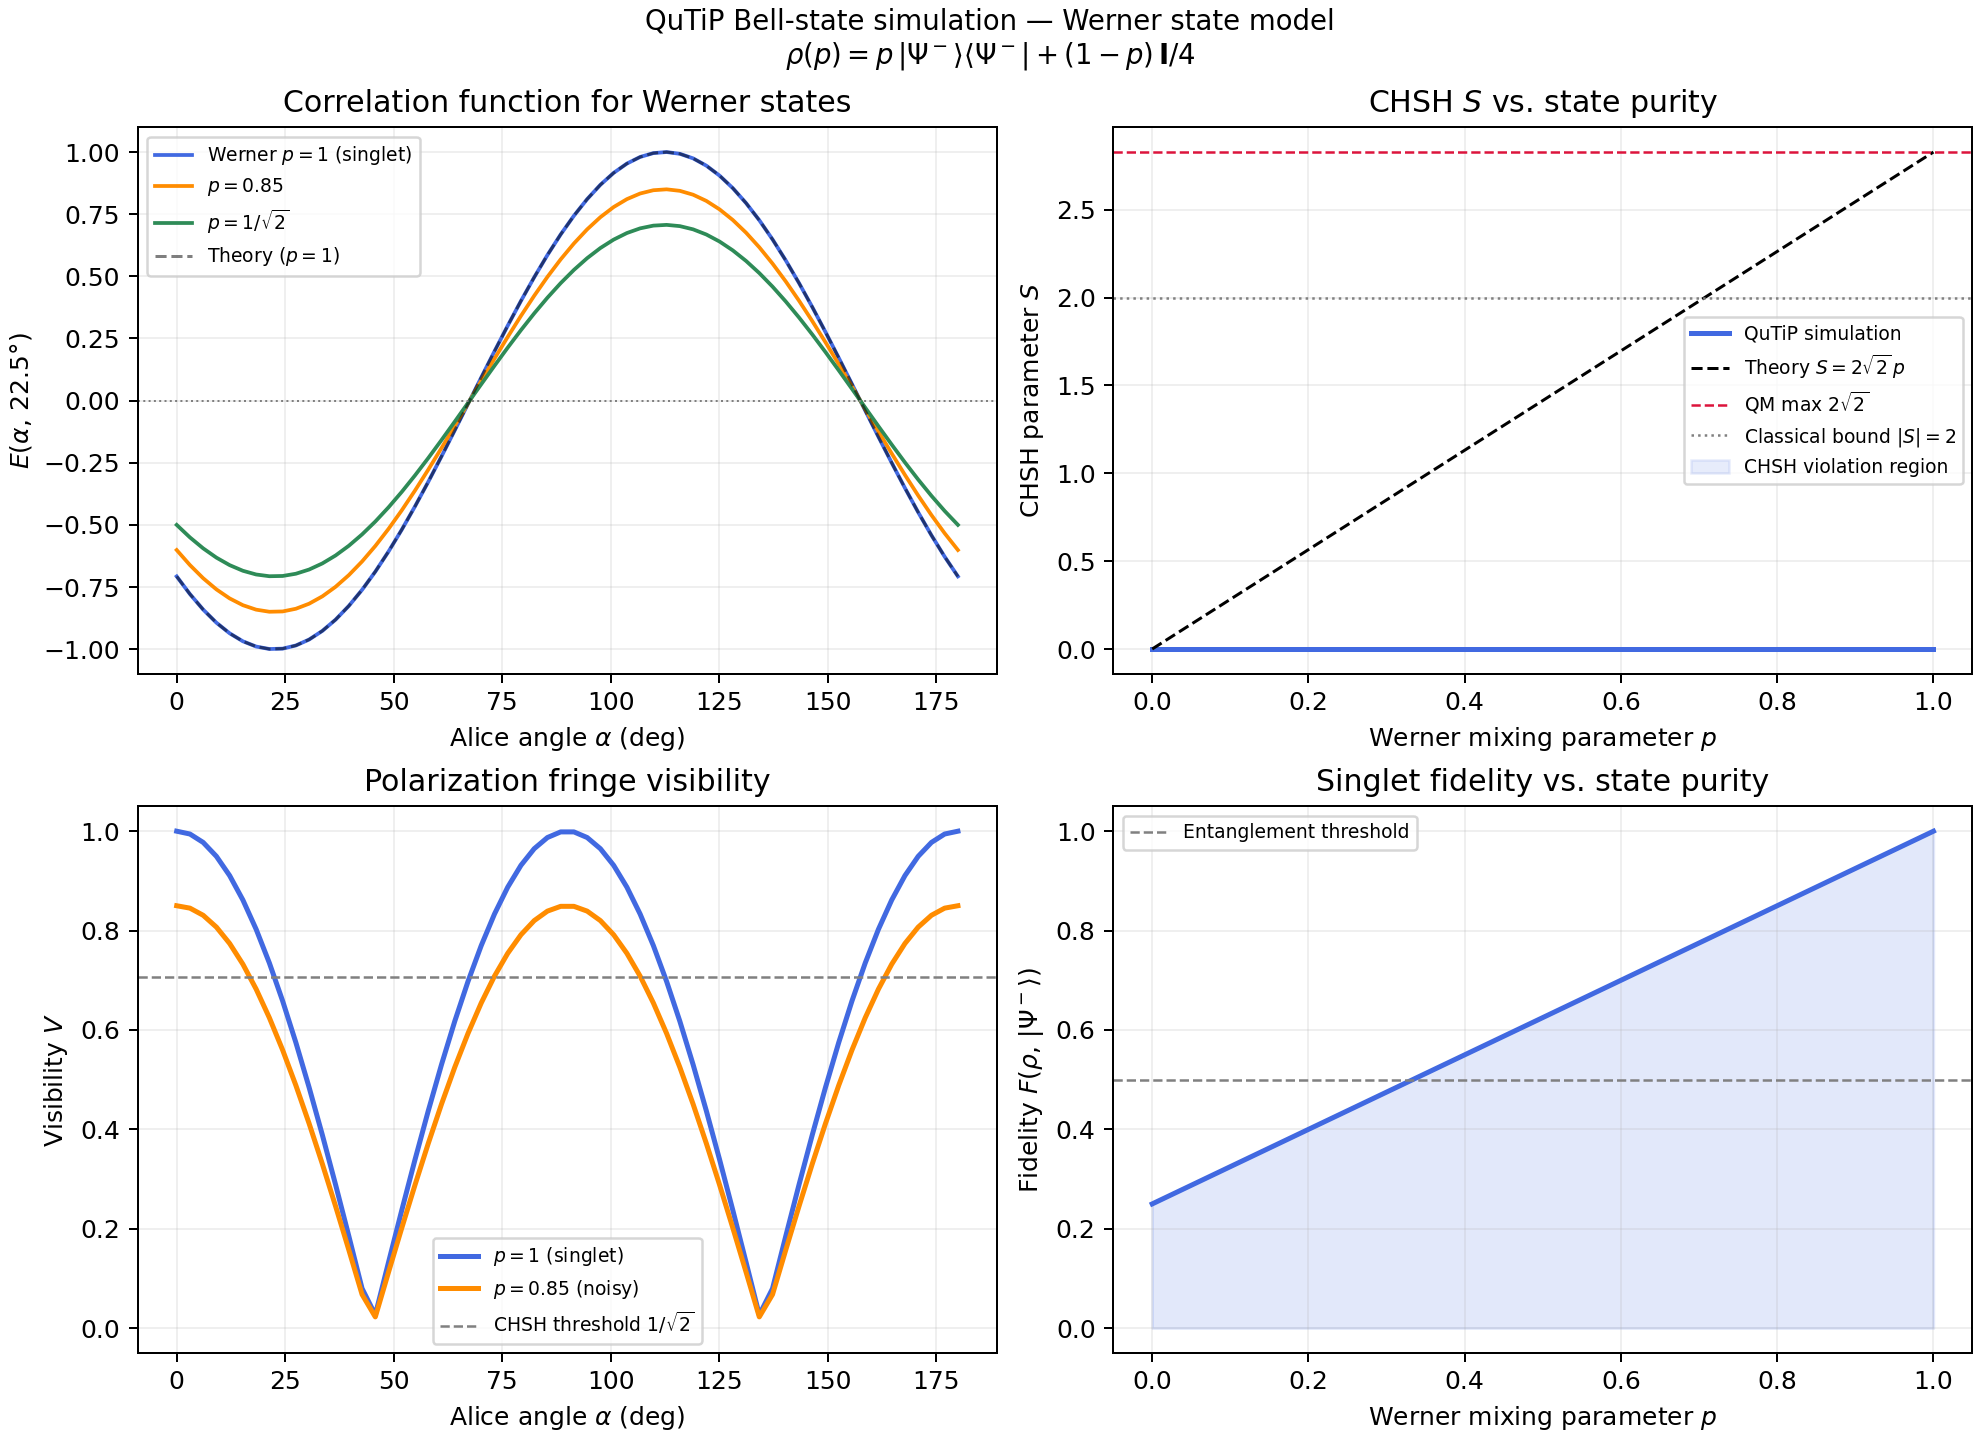
\includegraphics[width=\linewidth]{plots/qutip_bell_simulation.png}
    \caption{%
      QuTiP simulation of the Werner-state model
      $\rho(p)=p\,|\Psi^-\rangle\langle\Psi^-|+(1-p)\,\mathbf{I}/4$.
      \textbf{(a)} Correlation function $E(\alpha, 22.5^\circ)$ vs.\ Alice angle
      for $p\in\{1,\,0.85,\,1/\!\sqrt{2}\}$.
      \textbf{(b)} CHSH parameter $S$ vs.\ mixing parameter $p$; shaded region
      marks the $|S|>2$ quantum violation.
      \textbf{(c)} Polarization fringe visibility $V(\alpha)$ for the singlet
      and a noisy Werner state.
      \textbf{(d)} Fidelity $F(\rho,|\Psi^-\rangle)$ vs.\ $p$.%
    }
    \label{fig:qutip-sim}
\end{figure}

% (Notebook fragments are included at the end of the Appendix)

% ─── Results tables (auto-updated from analysis CSVs) ────────────────────────
% \csvdatatable{data/results_example.csv}%
%   {Caption describing the table contents.}%
%   {tab:example}%
%   {lrr}%
%   {Quantity \& Value \& Uncertainty \\\midrule}%
%   {\csvcoli \& \csvcolii \& \csvcoliii}

\subsection{Analysis Code}

\subsubsection*{Snakemake Pipeline Script}
The following functions from \texttt{pycode/generate\_long\_run\_plot.py} implement
the Werner-state QuTiP simulation that produces Fig.~\ref{fig:qutip-sim}.
Each function is shown as a separate listing to keep the display manageable.

\pysnippetmethod[Werner state density matrix $\rho(p)$.]{pycode/generate_long_run_plot.py}{werner_state}{code:fn-werner}

\pysnippetmethod[Two-photon polarization projector $\Pi(\theta,\varphi)$.]{pycode/generate_long_run_plot.py}{two_photon_projector}{code:fn-projector}

\pysnippetmethod[Coincidence rate $R(\alpha,\beta)$ from density matrix.]{pycode/generate_long_run_plot.py}{coincidence_rate}{code:fn-rate}

\pysnippetmethod[Normalized correlation function $E(\alpha,\beta)$.]{pycode/generate_long_run_plot.py}{E_from_rho}{code:fn-E}

\pysnippetmethod[CHSH parameter $S$ from density matrix.]{pycode/generate_long_run_plot.py}{CHSH_S_from_rho}{code:fn-chsh}

\pysnippetmethod[Fidelity to the singlet state $|\Psi^-\rangle$.]{pycode/generate_long_run_plot.py}{fidelity_to_singlet}{code:fn-fidelity}

\pysnippetmethod[Simulation: Correlation $E(\alpha, 22.5^\circ)$.]{pycode/generate_long_run_plot.py}{simulate_correlation}{code:fn-sim-corr}
\pysnippetmethod[Simulation: CHSH $S$ vs Purity $p$.]{pycode/generate_long_run_plot.py}{simulate_chsh}{code:fn-sim-chsh}
\pysnippetmethod[Simulation: Fringe Visibility $V(\alpha)$.]{pycode/generate_long_run_plot.py}{simulate_visibility}{code:fn-sim-vis}
\pysnippetmethod[Simulation: Fidelity to Singlet.]{pycode/generate_long_run_plot.py}{simulate_fidelity}{code:fn-sim-fid}

\pysnippetmethod[Plotting: Correlation panel.]{pycode/generate_long_run_plot.py}{plot_correlation}{code:fn-fig-corr}
\pysnippetmethod[Plotting: CHSH $S$ panel.]{pycode/generate_long_run_plot.py}{plot_chsh}{code:fn-fig-chsh}
\pysnippetmethod[Plotting: Visibility panel.]{pycode/generate_long_run_plot.py}{plot_visibility}{code:fn-fig-vis}
\pysnippetmethod[Plotting: Fidelity panel.]{pycode/generate_long_run_plot.py}{plot_fidelity}{code:fn-fig-fid}

\subsubsection*{Notebook Output Figures}
% Run the extraction script once, then uncomment % auto_nb_figures.tex — generated by nb_to_report.py
% Place % auto_nb_figures.tex — generated by nb_to_report.py
% Place % auto_nb_figures.tex — generated by nb_to_report.py
% Place \input{auto_nb_figures} inside Results section.
 inside Results section.
 inside Results section.
:
%   python3 pycode/nb_to_report.py pycode/optical_simulator.ipynb
% Produces auto_nb_figures.tex — one \begin{figure} block per output cell.
% auto_nb_figures.tex — generated by nb_to_report.py
% Place % auto_nb_figures.tex — generated by nb_to_report.py
% Place % auto_nb_figures.tex — generated by nb_to_report.py
% Place \input{auto_nb_figures} inside Results section.
 inside Results section.
 inside Results section.


\subsubsection*{Notebook Code Cells}
% After running nb_to_report.py above, auto_nb_code.tex contains the
% source of each code cell as a \begin{Code}...\end{Code} float.
% auto_nb_code.tex — generated by nb_to_report.py
% Place % auto_nb_code.tex — generated by nb_to_report.py
% Place % auto_nb_code.tex — generated by nb_to_report.py
% Place \input{auto_nb_code} inside Analysis Code section.

\paragraph{Setup}
\begin{Code}[H]
  \lstinputlisting[language=Python]{pycode/nb_cells/_nb_setup.py}
  \caption*{Notebook cell: Setup}
\end{Code}

\paragraph{Computation}
\begin{Code}[H]
  \lstinputlisting[language=Python]{pycode/nb_cells/_nb_computation.py}
  \caption*{Notebook cell: Computation}
\end{Code}
 inside Analysis Code section.

\paragraph{Setup}
\begin{Code}[H]
  \lstinputlisting[language=Python]{pycode/nb_cells/_nb_setup.py}
  \caption*{Notebook cell: Setup}
\end{Code}

\paragraph{Computation}
\begin{Code}[H]
  \lstinputlisting[language=Python]{pycode/nb_cells/_nb_computation.py}
  \caption*{Notebook cell: Computation}
\end{Code}
 inside Analysis Code section.

\paragraph{Setup}
\begin{Code}[H]
  \lstinputlisting[language=Python]{pycode/nb_cells/_nb_setup.py}
  \caption*{Notebook cell: Setup}
\end{Code}

\paragraph{Computation}
\begin{Code}[H]
  \lstinputlisting[language=Python]{pycode/nb_cells/_nb_computation.py}
  \caption*{Notebook cell: Computation}
\end{Code}


% ===========================================================================
\section{Conclusion}
% ===========================================================================
\begin{guidance}
\textit{\color{gray!60!black}\small\textbf{Conclusion guidance:}
  For each key result:
  \begin{itemize}[noitemsep,topsep=2pt]
    \item Quote the measured value $\pm$ uncertainty.
    \item Compare to theoretical expectation and state agreement/disagreement.
    \item Discuss dominant error sources and how they could be reduced.
  \end{itemize}
  Conclude with the physical significance of the findings.}
\end{guidance}
[Insert Conclusion Here]

% ===========================================================================
% \nocite{*} makes ALL entries in refs.bib appear in the bibliography,
% even if not explicitly cited in the text. Remove it once you add real \cite{} calls.
\nocite{*}
\printbibliography
% ===========================================================================

\end{document}
